\documentclass[conference]{IEEEtran}
\usepackage{cite}
\usepackage{amsmath,amssymb,amsfonts}
\usepackage{algorithmic}
\usepackage{graphicx}
\usepackage{textcomp}
\usepackage{xcolor}
\usepackage{colortbl}
\usepackage{multirow}
\usepackage[export]{adjustbox}
\def\BibTeX{{\rm B\kern-.05em{\sc i\kern-.025em b}\kern-.08em
    T\kern-.1667em\lower.7ex\hbox{E}\kern-.125emX}}
\begin{document}
\title{
    What is good project methodology for small IT-projects?\\
{\normalsize An attempt to answer this in course II1302 "Projekt och projektmetoder"
at KTH EECS Kista the Spring 2022}

% To accommodate for the .doc's formatting, the author blocks have been replaced with this section instead.
\begin{center}
    \large{ 
        Arif Jehda-Oh\textsuperscript{1}, Caroline Gross Liljenström\textsuperscript{2}, Gustav Normelli\textsuperscript{3}, Jesper Jansson\textsuperscript{4}, Natasha Donner\textsuperscript{5}, Wilhelm Nordgren\textsuperscript{6}\\
        \textit{\\EECS, KTH\\
                Kistagången 16, 164 40 Kista, Sweden\\}
        \textsuperscript{1}\texttt{arifjo@kth.se}\\
        \textsuperscript{2}\texttt{}\\
        \textsuperscript{3}\texttt{normelli@kth.se}\\
        \textsuperscript{4}\texttt{jespja@kth.se}\\
        \textsuperscript{5}\texttt{ndonner@kth.se}\\
        \textsuperscript{6}\texttt{}\\
        
        %\textit{Second Company\\
        %Address Including Country Name\\}
        %\textsuperscript{2}\texttt{second.author@second.com}
    }
\end{center}
}

% This is just to kill the warning about no author given.
\author{}




\maketitle

\begin{abstract}
Syfte och mål med kursen - "Vad är en bra projektmetod för små IT-projekt?" Kursens metod för att uppnå
kursens syfte och mål. Resultat av kursens metod - uppfylls syfte och mål med kursen.\\
Kan undersökningsfrågan besvaras?

What is a good project method for small IT projects? 

To give students the knowledge and brief experience about project methods used in small IT projects ... Role play ... seminar etc ...

This method gives the students a good knowledge and a somewhat ____ experience in ... However other methods are not tested = students can only say if his or her group used the SCRUM method in a way that felt good for him or her, not if any other would have worked better, if _____ or if they even followed the SCRUM method as it is supposed/meant to. 


\end{abstract}

\begin{IEEEkeywords}
Group project, IoT, Project method, Scrum, KTH EECS. 
\end{IEEEkeywords}

\section{Om detta dokument och undersökning}
Vem är läsaren? Dokumentets disposition (istället för innehållsförteckning). Vilken trovärdighet har innehållet?

Testar att citera \cite{eklund_arbeta_2010}

Projektets resultat (framtagen produkt) framgår av bilagorna.

Bilagor.

\section{Introduction}
Om detta kapitel \dots

\subsection{Background}
Mer om kursen, syfte och mål. Allmänt om IT-projekt. Undersökningsfrågan.

\subsection{Problem Statement}
Övergripande frågeställning.
Vad menas med en bra projektmetod? Åstadkommer/skapar projeket rätt saker och konstrueras
lösningar på bästa sätt?

\subsection{Investigation Strategy}
Fallstudie genom att i grupp försöka genomföra ett mindre IT-projekt med utvalda projektmetoder
och där varje gruppmedlem värderar sitt ansvarsområde i projektet för att ur detta försöka
besvara den övergripande frågeställningen.

\subsection{Related}
Lorem ipsum.

\subsection{Restrictions and Limitations}
Dolor sit.
\section{Teori och ingenjörspraxis.}
Detta kapitel listar och i viss mån beskriver teorier och ingenjörspraxis som använts
i undersökningen. Det finns två underkapitel, litteraturstudie och förstudie.

\subsection{Litteraturstudie.}
I detta kapitel anges litteratur och andra källor som har använts för att hitta ingångar
och möjligheter i undersökningen. Förutom de källor som anges finns förmodligen andra 
och kanske bättre källor som denna studie inte använt sig av.

Undersökningen görs utifrån övergripande projektmetoder men också utifrån specifika metoder
och arbetssätt som används av olika kompetenser i projektets team. Vilka dessa kompetenser
är framgår av texten nedan.

\textbf{Övergripande källor}
\begin{itemize}
    \item Projektets hälsa och status
    \item Scrum
    \item Fasindelning
    \item Projektgrunder
    \item Person och gruppdynamik
\end{itemize}

\textbf{Kundrepresentant} - kompetens enligt [Essence 1.0]
\begin{itemize}
    \item Vision
    \item Kravspecifikation
    \begin{itemize}
        \item "Stories
        \item "UseCase"
    \end{itemize}
\end{itemize}

\textbf{Analytiker} - kompetens enligt ...
\begin{itemize}
    \item Arkitektur (Kruchten, 1995)
\end{itemize}

\textbf{Utvecklare} - kompetens enligt ...
\begin{itemize}
    \item Designplan
\end{itemize}

\textbf{Testare} - kompetens enligt ...
\begin{itemize}
    \item Testplan
\end{itemize}

\textbf{Ledning och styrning} - kompetens enligt ...
\begin{itemize}
    \item Projektplanering
    \begin{itemize}
        \item Projektdefinitionen
    \end{itemize}
\end{itemize}

\textit{\textbf{Miljö, hållbar utveckling, etik och jämställdhet}}

\textit{\textbf{Arbetsmiljö}}

\subsection{Förstudie}
Vilka möjligheter till ansats har beaktats och prövats? Brett perspektiv.
Enligt undersökningsstrategin så skall någon projektmetod prövas i ett 
praktiskt projekt och utifrån de erfarenheter som fås görs en värdering
av använda metoder. Frågan är då vilken ansats av projektmetod som skall 
användas. Eftersom erfarenheten av projektarbete hos studenterna i denna 
kurs är liten så fanns det ett färdigt förslag till ansats av projektmetod. 
Detta projektmetodförslag kan senare modifieras av projektgruppen.
Tidigare kursomgångar och lärarens förslag har mynnat ut i följande ansats.
Projektmetoden framgår med god tydlighet av de arbetstavlor som definierats 
i ansatsen, se figurer och bilder.
Vision, projektdefinition, iterativt, Scrum ….
Resultatet av förstudien är att metoderna, som anges i följande kapitel,
har valts för undersökningens genomförande.\\

\begin{enumerate}
    \item \textit{Arbetstavla}
    \begin{figure}[htbp]
        \centerline{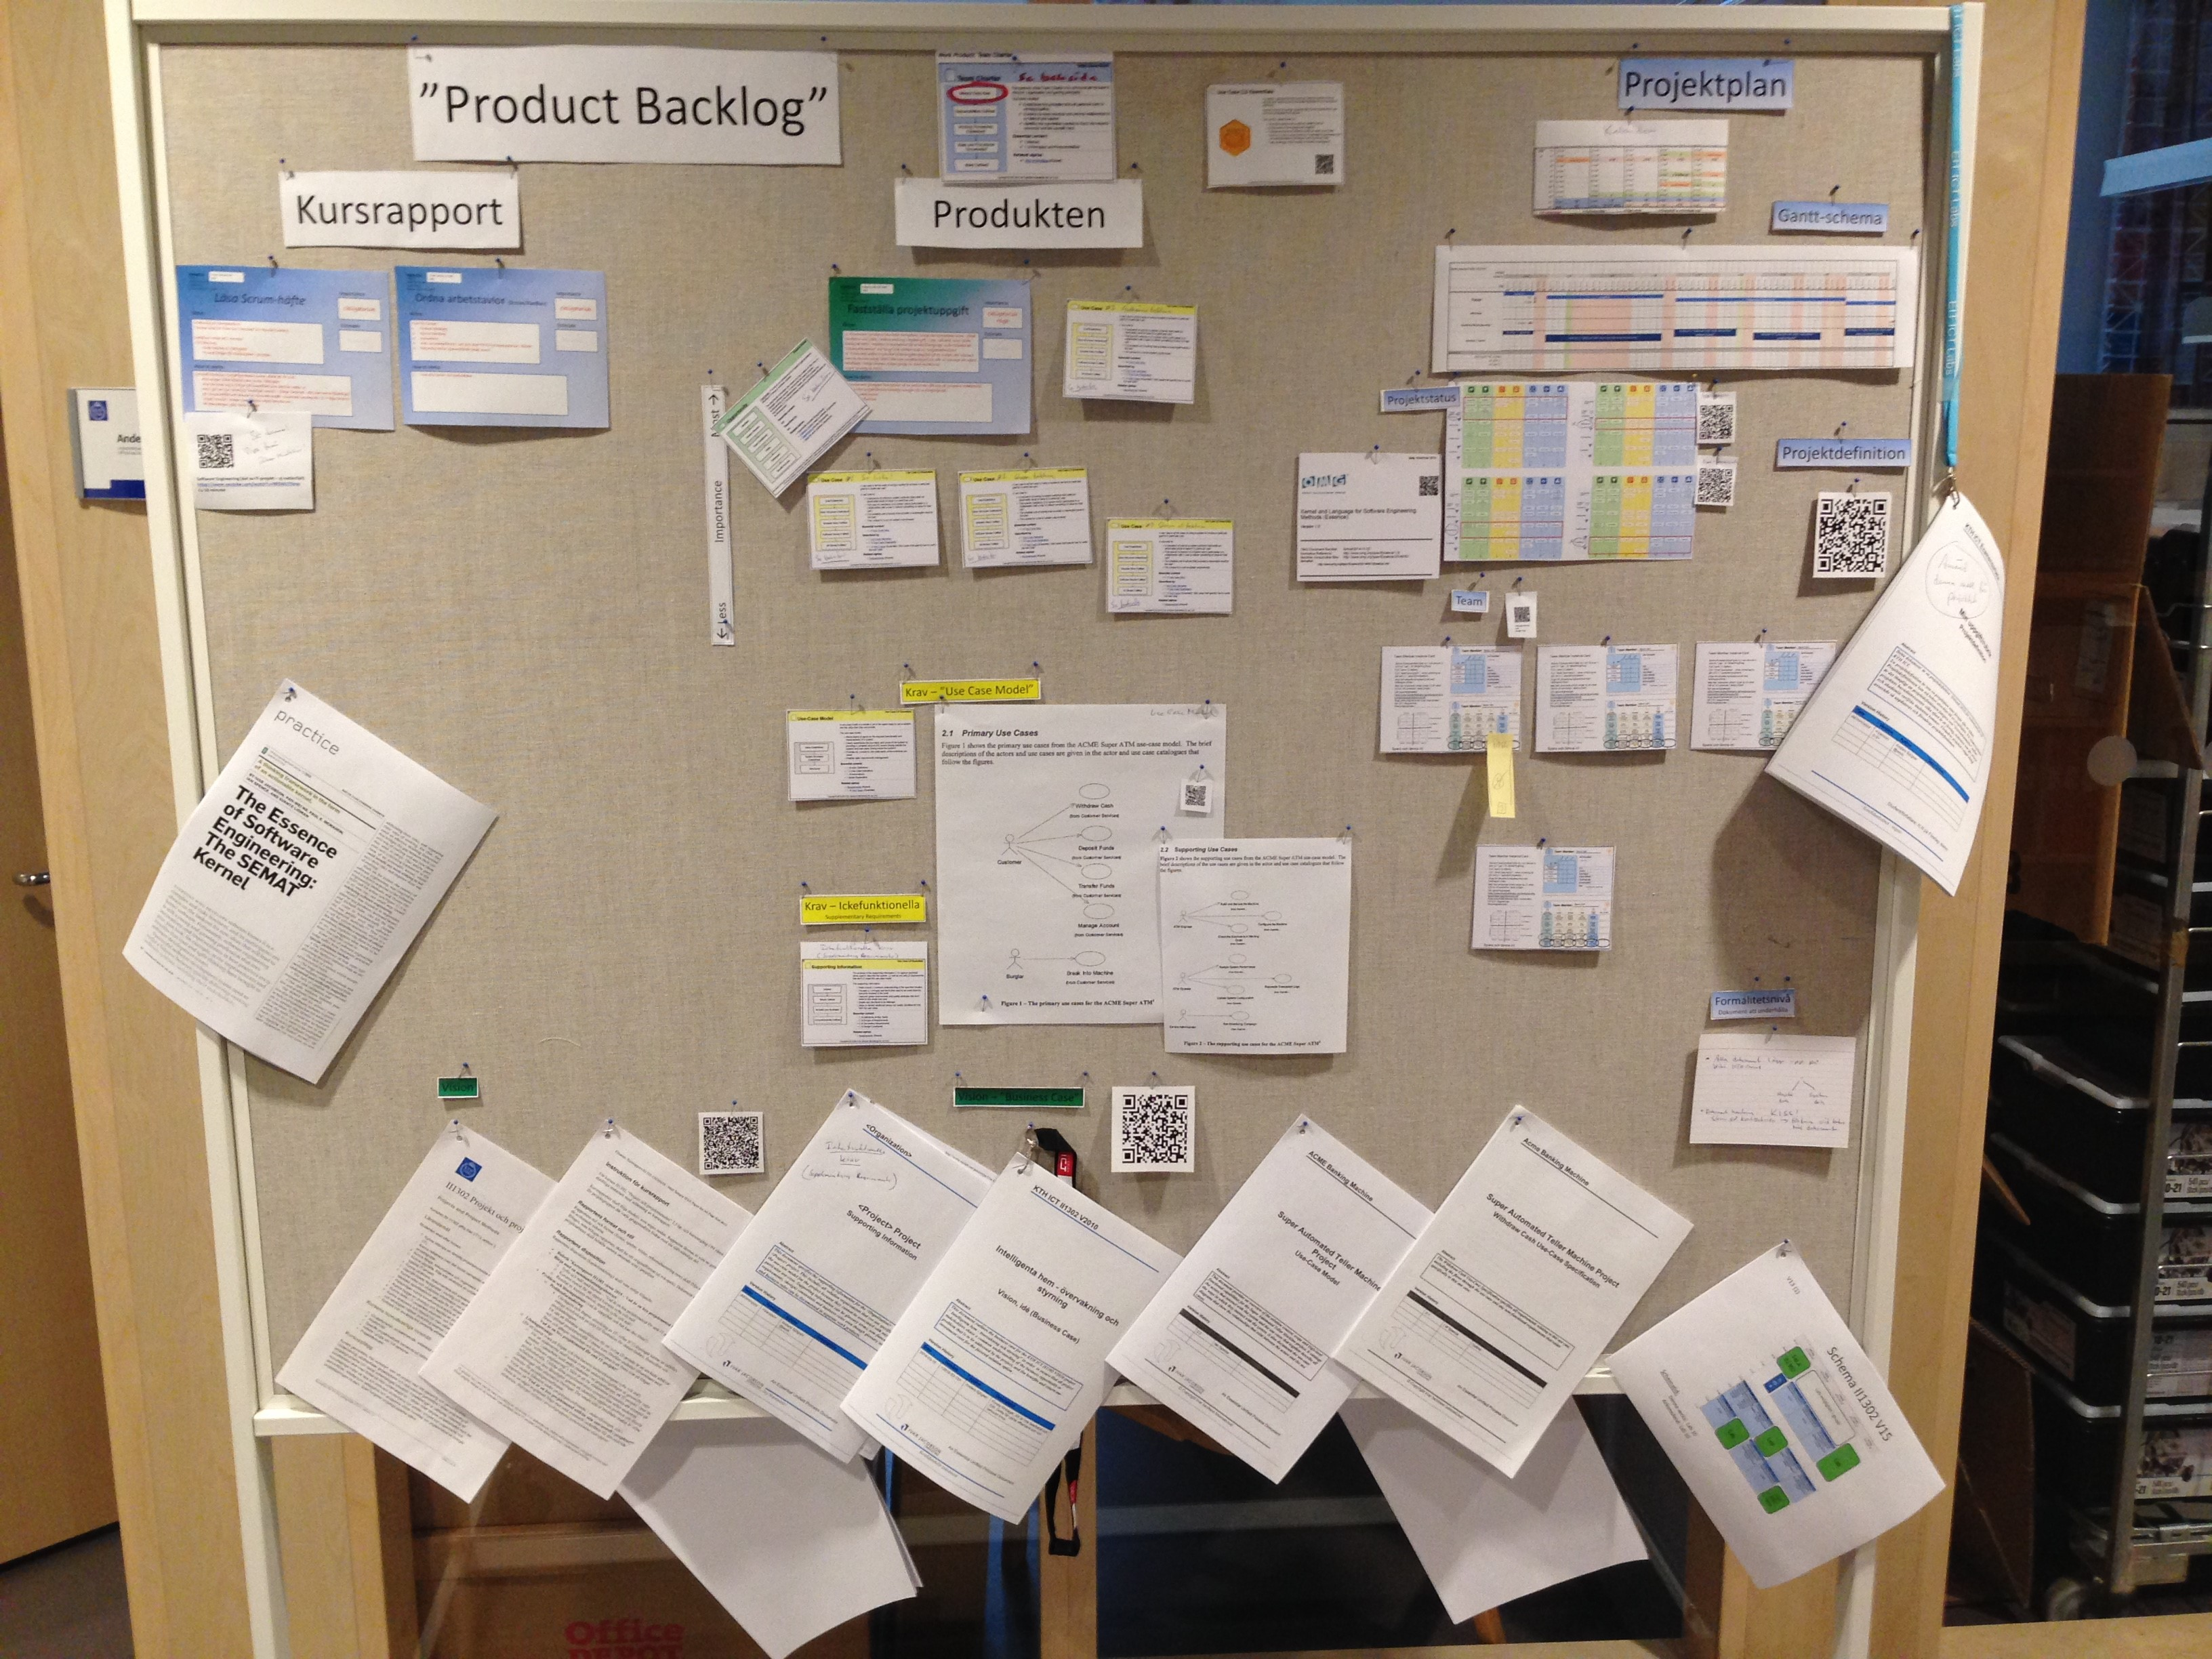
\includegraphics[max height=250px, max width=250px]{Z. images/arbetstavla.jpg}}
        \caption{Arbetstavla "nåldyna"}
        \label{fig}
    \end{figure}
    
    \begin{figure}[htbp]
        \centerline{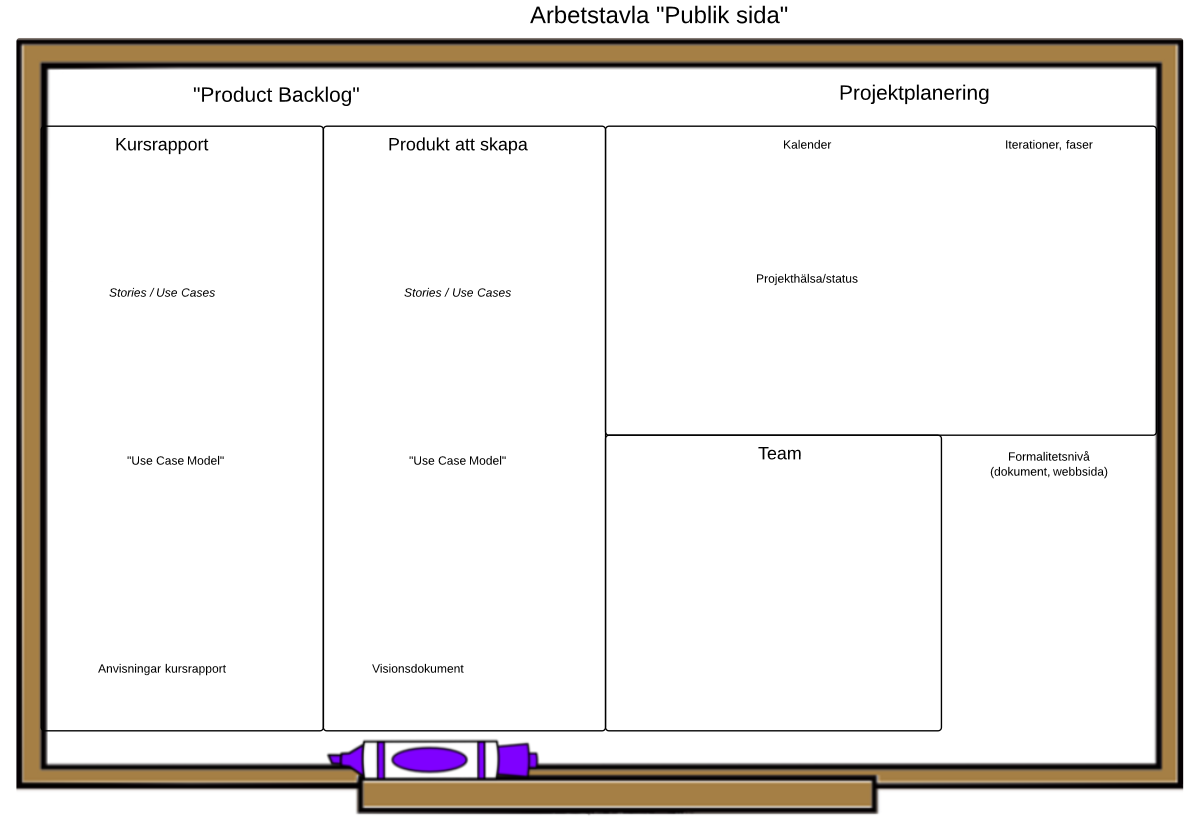
\includegraphics[max height=250px, max width=250px]{Z. images/lucidtavla.png}}
        \caption{Arbetstavla "whiteboard" "Publik sida"}
        \label{fig}
    \end{figure}

    \begin{figure}[htbp]
        \centerline{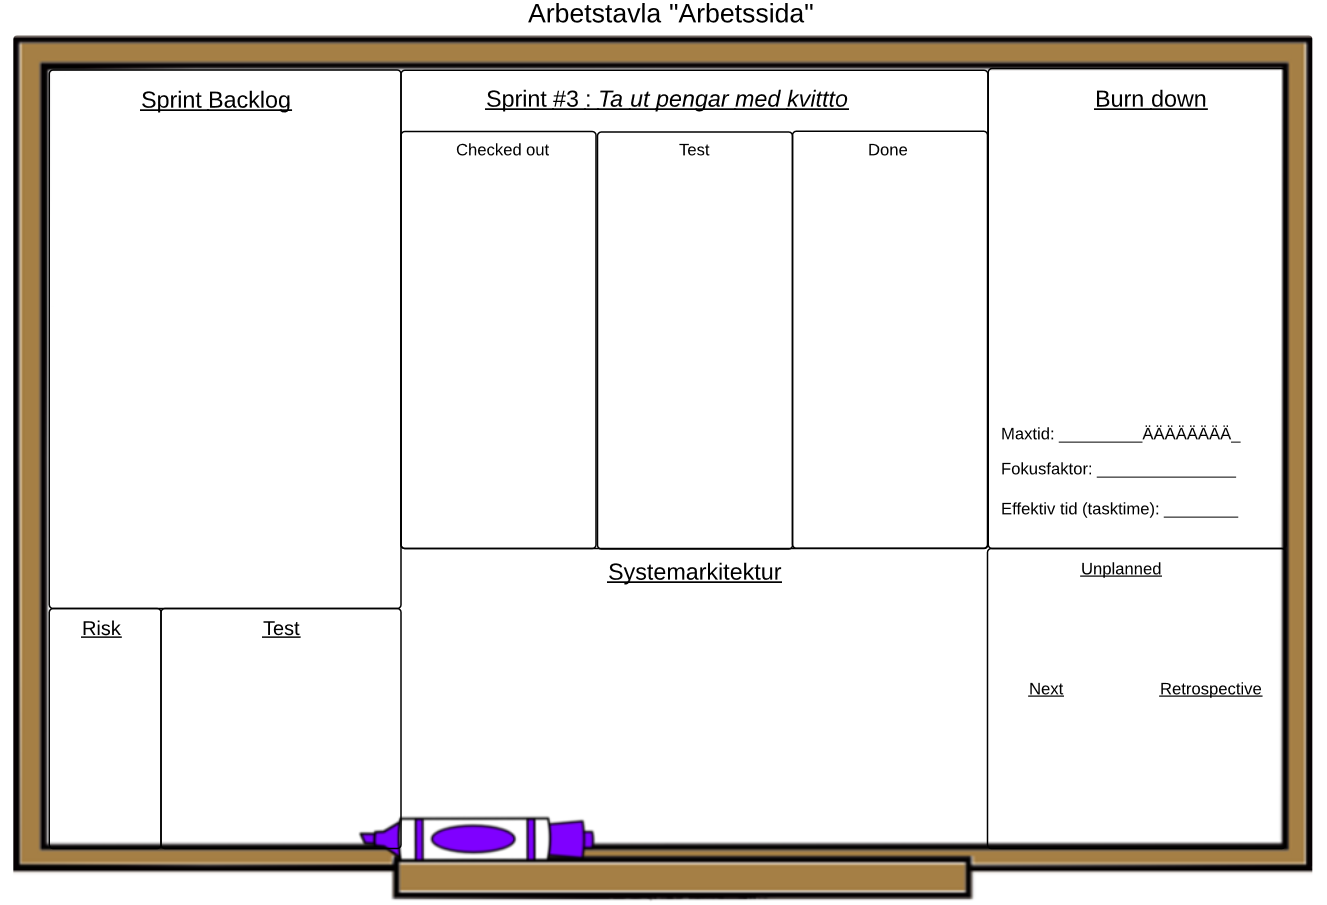
\includegraphics[max height=250px, max width=250px]{Z. images/lucidbaksida.png}}
        \caption{Arbetstavla "whiteboard" "Arbetssida"}
        \label{fig}
    \end{figure}
    \item \textit{Scruminspirerade projektaktiviteter}
    Bilden nedan visar projektmodellens aktiviteter och ordning.

    \begin{figure}[htbp]
        \centerline{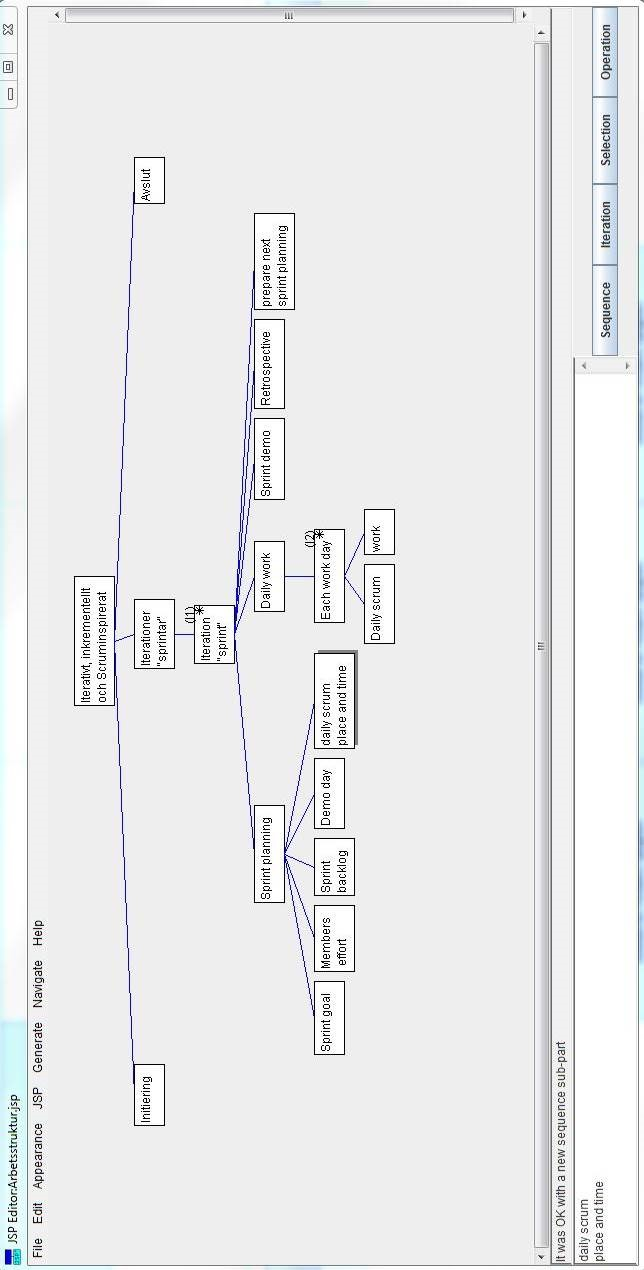
\includegraphics[max height=250px, max width=250px]{Z. images/scrum.jpg}}
        \caption{Den här har ingen beskrivning i mallen.}
        \label{fig}
    \end{figure}
\end{enumerate}
\section{Research Methods}


The research methods describe the methods that will answer the main research question, listed below and followed by a method description of the different project methods.


\subsection{Questions to be answered in the research}

\begin{enumerate}
    \item{How should one assess\/report whether some project method or practicum is suitable for an IoT project?}
    \item{How to categorize, select and name project methods?}
    \item{What are the responsibility roles used in a project?}
    \item{What is a project built of, and which methods/practices for examining and asserting the knowledge?}
\end{enumerate}

\subsection{Method Description}

In this section we describe the different project methods, and the methods that are used in the project.
The two common methods are the \textit{SCRUM} and the \textit{Kanban} method.
Both methods are based on the same principles, but the SCRUM method is more formal structure that focuses on the development of the project, while the Kanban method focuses on the implementation of the project.
The difference between the two methods is that the SCRUM method is based on the \textit{Sprint} concept, while the Kanban method is based on the \textit{Task} concept.

Scrum\cite{atlassianScrum} is build upon a structure of \textit{Sprints}, which are defined by the \textit{Sprint Goal}, \textit{Sprint Backlog}, \textit{Sprint Review} and \textit{Sprint Retrospective}.
Sprint goal, is about the project's main goal, while the Sprint Backlog is a list of the tasks that need to be done in the Sprint.
The workboard is build on states which the tasks are in, and the workboard is used to show the progress of the project and the board is generated for every iteration.
The workboard coloums states are:
\begin{enumerate}
    \item{To Do}
    \item{In Progress}
    \item{In Review}
    \item{Done}
\end{enumerate}

The Sprint Retrospective is a list of the tasks that were done in the Sprint, and the Sprint Review is a list of the tasks that were not done in the Sprint.
The retrospective is about understanding the why and how the tasks were completed.
During the retrospective you state what was good, what was bad, what could be improved and what could be done better, and implement the changes into the next Sprint.


The Kanban\cite{atlassianKanban} method is based on the \textit{Task} concept, which is defined by the \textit{Task Board}, \textit{Task Backlog}, \textit{Task Review} and \textit{Task Retrospective}.
The Task Board is a list of the tasks that need to be done in the project.
The Task Backlog is a list of the tasks that are in progress.
The Task Review is a list of the tasks that were done in the project and are waiting for review.
The Task Retrospective is a list of the tasks that were done in the project, and the Task Review is a list of the tasks that were not done in the project.

The concept of Kanban and Scrum is very similiar as described above.


As the course material and course requirements were optimized for utilizing the Scrum\cite{atlassianScrum} method, with all the iterations and their requirements for each iteration.
The course material is divided into the following sections:
\begin{enumerate}
    \item{Iteration 1, Introduction of course and project requirements.}
    \item{Iteration 2, Elaboration of the project requirements.}
    \item{Iteration 3, Construction of the project requirements.}
    \item{Iteration 4, Construction of the project requirements.}
    \item{Iteration 5, Transition of the project requirements.}
\end{enumerate}

The project group members was divided into the following groups:
\begin{enumerate}
    \item{Project Manager, was tasked to be responsible for the presentation of the product and write a documenation about the project definition.}
    \item{Customer and Requirements Manager, was tasked to be responsible for the defining the vision and business case with the product is going to be fulfill.}
    \item{Architecture, was tasked to come up with a architecture for the whole product.How all the components communicate with the others modules which then leads to the end product primary use case.}
    \item{Construction and development Manager, is responsible for writing a component description that are based on the architectual design.}
    \item{Test Manager, is responsible for creating test cases which full fufill the use case defined in the project.}
    \item{Sustainability\/Work Environment Manager, is responsible for creating a sustainability development description.}
\end{enumerate}


In this course the project group focus on the Scrum\cite{atlassianScrum} method for developing the product.
For structuring the project the project group implemented the workboard in GitHub Project Management tool\cite{github-project-board}.
The workboard was divided into different tabs which provided different information to the external viewers and the project members.
The workboard tabs was divided into the following tabs:
\begin{enumerate}
    \item{Project Planner List, used for an overview of all task in the project with detailed metadata.}
    \item{Project Planner Table, used for external presentation of the project plan and their sprint goals.}
    \item{Current Sprint List, used for an overview of all task in the current sprint with detailed metadata.}
    \item{Current Sprint Table, used for external presentation of the current sprint plan and their sprint progress.}
    \item{My To Do's, filtered tasks which have been assigned to a specific user.}
    \item{Stories Table, used for having an overview of all task connected to a specific story.}
\end{enumerate}

Every iteration was followed by a sprint planning meeting, where the group stated the sprint goals, and the sprint backlog for the iteration.
The sprint ended with a sprint demo of the current iteration progress, the sprint retrospective of the iteration progress, and a Game Score Card for grading the performance on itself and on the project members. 

\section{Implementation}
I följande kapitel redovisas viktiga beslut, förändringar och anpassningar som gjorts 
i projektmetod, projektpraktiker, värderingar, beslut mm som gjorts under studiens genomförande.
(Här kan det vara lämpligt med en indelning i olika ansvarsområden inom projektet?)

\subsection{Projektledning (Stina)}
Genomförandet av iterationer följer helt och hållet mallen för s k ”sprint” i Scrum [ref] 
och beskrivs enklast med följande aktivitetsdiagram, se  bild
\begin{figure}[htbp]
    \centerline{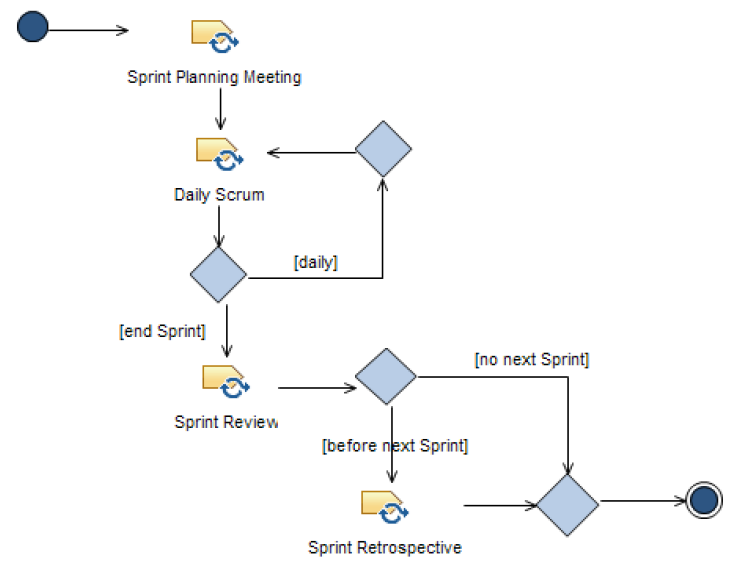
\includegraphics[max height=250px, max width=250px]{Z. images/sprint.png}}
    \caption{Iteration/Sprint}
    \label{fig}
\end{figure}

\subsection{Kundrepresentant (Kurs)}
Lite innehåll.


\section{Result}
% Tabellen nedan listar bedömda ”områden” och subjektiv värdering gentemot deras bidrag 
% till Åstadkommer/skapar projektet rätt saker (validitet) och konstrueras lösningar på 
% bästa sätt (reliabilitet)? Alternativa arbetssätt och del-projektmetoder anges också.

% Fullständiga tabeller finns i bilagor. Där finns också den evidens som ligger till 
% grund för listade omdömen. Positiva omdömen anges med grönt, negativa med rött och 
% neutrala omdömen med gult. 
During the project a number of different methods and practices were used to structure and guide the work within the project. These methods and practices varied in scope and area of application, ranging from initial definition of the project to structuring of the development process to finalizing development into a finished product. In order to ascertain which of these were suitable for use in small IT projects, they were all subjectively evaluated by the group. The results of this evaluation were then compiled into a table, shown here as Table \ref{tab-results}. Each method or practice was given a grade of either GOOD, MIXED or BAD and the grades color coded with green, yellow and red, respectively. For all non-good grades suggestions for alternative methods or practices were added.

% Here you can define your own colors to use in the table. 
\definecolor{green}{RGB}{146,208,80}
\definecolor{pink}{RGB}{251,212,180}
\definecolor{yellow}{RGB}{255,255,0}
\definecolor{grey}{RGB}{217,217,217}
\begin{table}[htbp]
\begin{center}
\caption{Method and practices evaluation results}
\label{tab-results}
\resizebox{\columnwidth}{!}{%
\begin{tabular}{llll}
\hline
\textbf{Area of responsibility} & \textbf{Methodology/Practice} & \textbf{Evaluation} & \textbf{Alternative method/practice}  \\ \hline
\rowcolor{grey} General                    &                                   &       &                                       \\
                           & Iterative work flow               & \cellcolor{green} GOOD  &                                       \\
                           & \textbf{Scrum}                    & \cellcolor{green} GOOD  &                                       \\
                           & - Board (Digital: GitHub)         & \cellcolor{green} GOOD  &                                       \\
                           & - Board (Physical: Whiteboard)    & \cellcolor{green} GOOD  &                                       \\
                           & - Daily stand-ups                 & \cellcolor{green} GOOD  &                                       \\
                           & - Iteration planning              & \cellcolor{green} GOOD  &                                       \\
                                & - Story/Task points           & \cellcolor{yellow} MIXED               & Not necessary for smaller IT-projects \\
                           & - Burndown chart                  & \cellcolor{green} GOOD  &                                       \\
                           & - Demos                           & \cellcolor{green} GOOD  &                                       \\
                           & - Retrospectives                  & \cellcolor{green} GOOD  &                                       \\
\rowcolor{grey} Project management         &                                   &       &                                       \\
                           & Gantt chart                       & \cellcolor{yellow} MIXED & Integrate timeline in Scrum board     \\
                           & Alpha States                      & \cellcolor{red} BAD   & Not necessary for smaller IT-projects \\
                           & Discord channels                  & \cellcolor{green} GOOD  &                                       \\
\rowcolor{grey} Customer relations/demands &                                   &       &                                       \\
                           & Vision                            & \cellcolor{green} GOOD  &                                       \\
                           & Use Cases                         & \cellcolor{green} GOOD  &                                       \\
\rowcolor{grey} Architecture               &                                   &       &                                       \\
                           & C4 Model                          & \cellcolor{green} GOOD  &                                       \\
                           & Use Case Models                   & \cellcolor{yellow} MIXED & Sliced use case model                 \\
\rowcolor{grey} Development                &                                   &       &                                       \\
                           & HW/SW teams                       & \cellcolor{green} GOOD  &                                       \\
                           & \textbf{GitHub}                   & \cellcolor{green} GOOD  &                                       \\
                           & - Dedicated repositories          & \cellcolor{green} GOOD  &                                       \\
                           & - Pull request method             & \cellcolor{green} GOOD  &                                       \\
                           & - Branches for tasks              & \cellcolor{green} GOOD  &                                       \\
                           & - Continuous integration/delivery & \cellcolor{green} GOOD  &                                       \\
                           & \textbf{Platforms}                &       &                                       \\
                           & - Heroku                          & \cellcolor{green} GOOD  &                                       \\
                           & - STM32CubeIDE                    & \cellcolor{yellow} MIXED & VSCode                                \\
\rowcolor{grey} Testing                    &                                   &       &                                       \\
                           & Test Driven Development           & \cellcolor{green} GOOD  &                                       \\ \hline
\end{tabular}%
}
\end{center}
\end{table}
During development, after each sprint, ways of working used during that sprint were brought up for scrutiny. This was done as a group exercise where group members were able to bring up certain ways of working that they felt needed to be focused on. It could either be to highlight something that was working well, to bring up something that needed to be changed or even stopped, or to propose something new that they felt was missing. In practice this was done by categorizing each of the things brought forward into either START, STOP or CONTINUE. The group would then address each of the added points in turn and discuss, if needed, a way to solve any issues identified with that particular point. For every new sprint the lists from the previous sprint were looked over and any points that still needed addressing were kept, and maybe re-categorized, or removed if the group felt it no longer needed addressing. In fact, even the method for this exercise was evaluated and changed between sprints, as the categories were at the first meeting defined as GOOD, COULD HAVE DONE BETTER and IMPROVEMENTS, but after the first two sprints it was decided to change them to START, STOP or CONTINUE because it was felt that this was a more concise way of naming them. The results of these exercises are presented here in Table \ref{tab-wow}.
\begin{table}[htbp]
\caption{Ways of working, SPRINTS 1-4}
\label{tab-wow}
\resizebox{\columnwidth}{!}{%
\begin{tabular}{lll}
\hline
\multicolumn{3}{c}{\rowcolor{grey} \textit{\textbf{SPRINT 1}}}                                                                              \\ \hline
\textbf{GOOD}                       & \textbf{COULD HAVE DONE BETTER}    & \textbf{IMPROVEMENTS}                            \\ \hline
Got of to a good start              & Product is not completelly defined & More efficient use if  time                      \\
Documents ready                     & Information is unclear             & The work board                                   \\
Everybody shows commitment          & Misguided work efforts             & More zealous use of Scrum method                 \\
Open discussion                     & Keeping deadlines                  & Powerpoint - begin sooner, different approach    \\
Participation                       & Work time                          & Expand system architecture                       \\
Responsability taken                & Daily Scrum meetings               & Add deadlines                                    \\
High pace                           &                                    & Read up on theory before starting practical work \\
Scrum                               &                                    & Collect documents in one file                    \\
                                    &                                    & Appoint tasks according to personal strengths    \\ \hline
\multicolumn{3}{c}{\rowcolor{grey} \textit{\textbf{SPRINT 2}}}                                                                              \\ \hline
\textbf{GOOD}                       & \textbf{COULD HAVE DONE BETTER}    & \textbf{IMPROVEMENTS}                            \\ \hline
Product completelly defined         & More focused work                  & Add more tasks to software team                  \\
Clearer information                 & More zealous use of Scrum method   & Demo: hardware before software                   \\
Deadlines                           & Tasks definition of done           & Alpha states                                     \\
Work time                           & Hardware teams use of GitHub       & Marry GitHub and CubeIDE                         \\
Daily Scrum meetings                & More clearly defined tasks         & Story points per member                          \\
More efficient use if  time         &                                    & Read up on theory before starting practical work \\
Powerpoint                          &                                    & Log progress in burndown right away              \\
Expanded system architecture        &                                    & Re-prioritize MuSCoW for hardware                \\
Collect documents in one file       &                                    &                                                  \\
Alot of progress with software      &                                    &                                                  \\
Burndown chart                      &                                    &                                                  \\
Progress with hardware              &                                    &                                                  \\
Demo                                &                                    &                                                  \\
Scrum board                         &                                    &                                                  \\
MuSCoW                              &                                    &                                                  \\
Finished 75\% of last sprint        &                                    &                                                  \\ \hline
\multicolumn{3}{c}{\rowcolor{grey} \textit{\textbf{SPRINT 3}}}                                                                              \\ \hline
\textbf{START}                      & \textbf{STOP}                      & \textbf{CONTINUE}                                \\ \hline
Acceptance criteria                 & Tasks \textless 4h                 & Prepare report                                   \\
Preparing Powerpoint earlier        & Tasks for reading up on theory     & Working in different teams                       \\
Better definition of tasks          &                                    & Sitting together                                 \\
- Naming                            &                                    & Read up on theory before starting coding         \\
- Checklist                         &                                    & Mob programming                                  \\
- Acceptance criteria               &                                    & Ask for help outside the group                   \\
Package IoT                         &                                    & Daily Scrum meetings                             \\
Subtasks if needed                  &                                    & Deadlines                                        \\
Log progress in burndown right away &                                    & Efficient use of work time                       \\
Balanced work time                  &                                    & Alpha states                                     \\
                                    &                                    & Agenda for group meetings                        \\ \hline
\multicolumn{3}{c}{\rowcolor{grey} \textit{\textbf{SPRINT 4}}}                                                                              \\ \hline
\textbf{START}                      & \textbf{STOP}                      & \textbf{CONTINUE}                                \\ \hline
Ask for help outside the group      & Getting stuck                      & Follow instructions                              \\
Planned milestones                  &                                    & Better definition of tasks                       \\
Implement "unplanned tasks"         &                                    & - Naming                                         \\
Evaluate time cost of task early    &                                    & - Checklist                                      \\
Log progress in burndown right away &                                    & - Acceptance criteria                            \\
Balanced work time                  &                                    & - Subtasks if needed                             \\
Efficient use of work time          &                                    & - Divide task points for subtasks?               \\
                                    &                                    & Deadlines                                        \\
                                    &                                    & Alpha states                                     \\
                                    &                                    & Daily Scrum meetings                             \\
                                    &                                    & MOB programming                                  \\
                                    &                                    & Read up on theory before starting coding         \\
                                    &                                    & Working in different teams                       \\
                                    &                                    & Sitting together                                 \\
                                    &                                    & Agenda for group meetings                        \\
                                    &                                    & Preparing Powerpoint earlier                    \\ \hline
\end{tabular}%
}
\end{table}
% \begin{table}[htbp]
% \caption{Ways of working, SPRINT 1}
% \label{tab-wow1}
% \resizebox{\columnwidth}{!}{%
% \begin{tabular}{lll}
% \hline
% \textbf{GOOD}              & \textbf{COULD HAVE DONE BETTER}    & \textbf{IMPROVEMENTS}                            \\ \hline
% Got of to a good start     & Product is not completelly defined & More efficient use if  time                      \\
% Documents ready            & Information is unclear             & The work board                                   \\
% Everybody shows commitment & Misguided work efforts             & More zealous use of Scrum method                 \\
% Open discussion            & Keeping deadlines                  & Powerpoint - begin sooner, different approach    \\
% Participation              & Work time                          & Expand system architecture                       \\
% Responsability taken       & Daily Scrum meetings               & Add deadlines                                    \\
% High pace                  &                                    & Read up on theory before starting practical work \\
% Scrum                      &                                    & Collect documents in one file                    \\
%                           &                                    & Appoint tasks according to personal strengths    \\ \hline
% \end{tabular}%
% }
% \end{table}
% \begin{table}[htbp]
% \caption{Ways of working, SPRINT 2}
% \label{tab-wow2}
% \resizebox{\columnwidth}{!}{%
% \begin{tabular}{lll}
% \hline
% \textbf{GOOD}                  & \textbf{COULD HAVE DONE BETTER}  & \textbf{IMPROVEMENTS}                            \\ \hline
% Product completelly defined    & More focused work                & Add more tasks to software team                  \\
% Clearer information            & More zealous use of Scrum method & Demo: hardware before software                   \\
% Deadlines                      & Tasks definition of done         & Alpha states                                     \\
% Work time                      & Hardware teams use of GitHub     & Marry GitHub and CubeIDE                         \\
% Daily Scrum meetings           & More clearly defined tasks       & Story points per member                          \\
% More efficient use if  time    &                                  & Read up on theory before starting practical work \\
% Powerpoint                     &                                  & Log progress in burndown right away              \\
% Expanded system architecture   &                                  & Re-prioritize MuSCoW for hardware                \\
% Collect documents in one file  &                                  &                                                  \\
% Alot of progress with software &                                  &                                                  \\
% Burndown chart                 &                                  &                                                  \\
% Progress with hardware         &                                  &                                                  \\
% Demo                           &                                  &                                                  \\
% Scrum board                    &                                  &                                                  \\
% MuSCoW                         &                                  &                                                  \\
% Finished 75\% of last sprint   &                                  &                                                  \\ \hline
% \end{tabular}%
% }
% \end{table}
% \begin{table}[htbp]
% \caption{Ways of working, SPRINT 3}
% \label{tab-wow3}
% \resizebox{\columnwidth}{!}{%
% \begin{tabular}{lll}
% \hline
% \textbf{START}                      & \textbf{STOP}                  & \textbf{CONTINUE}                        \\ \hline
% Acceptance criteria                 & Tasks \textless 4h             & Prepare report                           \\
% Preparing Powerpoint earlier        & Tasks for reading up on theory & Working in different teams               \\
% Better definition of tasks          &                                & Sitting together                         \\
% - Naming                            &                                & Read up on theory before starting coding \\
% - Checklist                         &                                & Mob programming                          \\
% - Acceptance criteria               &                                & Ask for help outside the group           \\
% Package IoT                         &                                & Daily Scrum meetings                     \\
% Subtasks if needed                  &                                & Deadlines                                \\
% Log progress in burndown right away &                                & Efficient use of work time               \\
% Balanced work time                  &                                & Alpha states                             \\
%                                     &                                & Agenda for group meetings                \\ \hline
% \end{tabular}%
% }
% \end{table}
% \begin{table}[htbp]
% \caption{Ways of working, SPRINT 4}
% \label{tab-wow4}
% \resizebox{\columnwidth}{!}{%
% \begin{tabular}{lll}
% \hline
% \textbf{START}                      & \textbf{STOP} & \textbf{CONTINUE}                        \\ \hline
% Ask for help outside the group      & Getting stuck & Follow instructions                      \\
% Planned milestones                  &               & Better definition of tasks               \\
% Implement "unplanned tasks"         &               & - Naming                                 \\
% Evaluate time cost of task early    &               & - Checklist                              \\
% Log progress in burndown right away &               & - Acceptance criteria                    \\
% Balanced work time                  &               & - Subtasks if needed                     \\
% Efficient use of work time          &               & - Divide task points for subtasks?       \\
%                                     &               & Deadlines                                \\
%                                     &               & Alpha states                             \\
%                                     &               & Daily Scrum meetings                     \\
%                                     &               & MOB programming                          \\
%                                     &               & Read up on theory before starting coding \\
%                                     &               & Working in different teams               \\
%                                     &               & Sitting together                         \\
%                                     &               & Agenda for group meetings                \\
%                                     &               & Preparing Powerpoint earlier             \\ \hline
% \end{tabular}%
% }
% \end{table}
% \begin{table}[htbp]
% \caption{Bedömningar}
% \begin{center}
% \begin{tabular}{|l|l|l|l|}
% \hline
% \textbf{Ansvars-}   & \textbf{Arbetssätt/metod}     & \textbf{Omdöme}       & \textbf{Alternativ} \\
% \textbf{område}     & \textbf{praktik/mönster}      & Fördelar och          & \\
%                     &                               & nackdelar             &  \\
% \hline
% Projekt-            &                               &                       & \\
% övergripande        &                               &                       & \\
% \hline
% Projekt-            &                               &                       & \\
% ledning             & Iterativt                     & \cellcolor{green}     & \\
% \hline
% Analytiker          & Arkitektur                    &                       & \\
% \hline
%                     &                               & \cellcolor{pink}      & \\
% \hline
%                     &                               & \cellcolor{yellow}    & \\
% \hline
%                     &                               &                       & \\
% \hline
% \end{tabular}
% \label{tab1}
% \end{center}
% \end{table}

% \begin{table}[htbp]
% \caption{"Keep - Problems - Try"\\\textit{Roll - student}}
% \begin{center}
% \begin{tabular}{|c|c|c|c|}
% \hline
% \multicolumn{4}{|c|}{\cellcolor{grey}\textbf{"Keep"}}\\
% \hline \rowcolor{grey}
% \textbf{"Keep"}                         & \textbf{Motivation}      & \textbf{Förbättringar} & \textbf{Referenser} \\
% \hline
%                                         &                          &                     & \\
%                                         &                          &                     & \\
% \hline
%                                         &                          &                     & \\
%                                         &                          &                     & \\
% \hline
%                                         &                          &                     & \\
% \hline
%                                         &                          &                     & \\
% \hline
%                                         &                          &                     & \\
% \hline
%                                         &                          &                     & \\
% \hline

% % This is a separator, since the tables in the .doc-template are labeled as the same table.
% \multicolumn{4}{c}{}\\

% \hline
% \multicolumn{4}{|c|}{\cellcolor{grey}\textbf{"Problems - Try"}}\\
% \hline \rowcolor{grey}
% \textbf{"Problem"}                      & \textbf{"Try what?}      & \textbf{Motivering} & \textbf{Referenser} \\
% \hline
%                                         &                          &                     & \\
%                                         &                          &                     & \\
% \hline
%                                         &                          &                     & \\
%                                         &                          &                     & \\
% \hline
%                                         &                          &                     & \\
% \hline
%                                         &                          &                     & \\
% \hline
%                                         &                          &                     & \\
% \hline
%                                         &                          &                     & \\
% \hline

% % This is a separator, since the tables in the .doc-template are labeled as the same table.
% \multicolumn{4}{c}{}\\

% \hline
% \multicolumn{4}{|c|}{\cellcolor{grey}\textbf{"Problems - Skip"}}\\
% \hline \rowcolor{grey}
% \textbf{"Problem"}                      & \textbf{"Skip or}        & \textbf{Motivering} & \textbf{Referenser} \\
% \rowcolor{grey}                         & \textbf{replace, why?"}  &                     &  \\
% \hline
%                                         &                          &                     & \\
%                                         &                          &                     & \\
% \hline
%                                         &                          &                     & \\
%                                         &                          &                     & \\
% \hline
%                                         &                          &                     & \\
% \hline
%                                         &                          &                     & \\
% \hline
%                                         &                          &                     & \\
% \hline
%                                         &                          &                     & \\
% \hline
% \end{tabular}
% \label{tab1}
% \end{center}
% \end{table}

\section{Analysis and Improvement}
Finns det förslag eller räcker resultaten ovan?


\section{discussion}
General discussion. What does the result say about "What is a good project method for small IT projects"?

The project group choose to strictly work by the Scrum Method. "Vad är problemställningen vi har?" Den rapporten som Arif delat med oss undersöker olika projektmetoder och diskuterar dessa här. Ska jag enbart diskutera Scrum? Vad tycler vi har varit dåligt/bra med Scrum. Jag tror personligen vi hade kunnat åstadkomma mer med en annan aproach men det är kanske inte gruppens generella åsikt.
Diskussionen ska byggas på resultatet så det behöver vara klart innan jag skriver!? 

\subsection{Method discussion}
Validity
Reliability

\subsection{Result discussion}
Validity
Reliability

\subsection{Bidrag till vetenskaplighet, ingenjörserfarenhet (studenterfarenhet?)}
Framtida förbättringar\dots

% A section marked with a * will not be numbered.
\section*{Slutord}
Eventuella slutord.

Berätta något om produkten ni konstruerade, ange en länk till projektets Github\cite{Eklund:2}, videopresentation?
Länka till Github, rapprt mm från ditt LinkedIn-konto som exempel på arbetsprover?\cite{DUMMY:1}

\vspace{12pt}

% You can switch citation style. ieeetran could be useful, as it is a bit more pleasing to the eyes.
\bibliographystyle{IEEEtran}
\bibliography{mainBibliograph}
\end{document}